\section{Background theory}
In telephone networks the dialed number is transmitted  with DTMF signals. Every number is  a result of two frequencies, as seen in  figure~\ref{fig:DTMF}. We used two algorithms that detected the vertical frequencies and 

\begin{figure}[H]
  \centering
  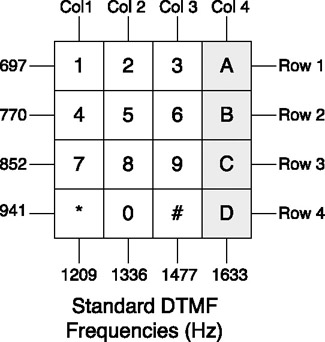
\includegraphics[width=0.8\linewidth]{DTMF}
  \caption{DTMF frequencies ~\cite{DTMF}}
\label{fig:DTMF}

\end{figure}